\section{Vectorization}\label{sec:vectorization}
Vectorization is a critical part of optimization; typically, vectorized code
can run many times faster than its un-vectorized counterpart. The reference
shallow simulator implemented in \ttt{central2d.h} is almost entirely
un-vectorized. For example, consider the loop in \figref{no-vec-code} which was
taken from \ttt{central2d.h}.

\begin{figure}[h]
\centering
\begin{CPP}[firstnumber=361]
// Copy from v storage back to main grid
for (int j = nghost; j < ny+nghost; ++j){
    for (int i = nghost; i < nx+nghost; ++i){
        u(i,j) = v(i-io,j-io);
    }
}
\end{CPP}
\caption{A loop from \ttt{central2d.h}.}
\label{fig:no-vec-code}
\end{figure}

The loop copies values from the \ttt{v} vector into the \ttt{u} vector; this is
clearly a vectorizable operation. However, consider the vectorization report in
\figref{no-vec-report}.

\begin{figure}[h]
\scriptsize
\begin{verbatim}LOOP BEGIN at central2d.h(362,5)
   #15344: loop was not vectorized: vector dep prevents vectorization
   #15346: vector dep: assumed FLOW dep between _M_elems line 364 and _M_elems line 364
   #15346: vector dep: assumed ANTI dep between _M_elems line 364 and _M_elems line 364

   LOOP BEGIN at central2d.h(363,9)
      #15344: loop was not vectorized: vector dep prevents vectorization
      #15346: vector dep: assumed FLOW dep between _M_elems line 364 and _M_elems line 364
      #15346: vector dep: assumed ANTI dep between _M_elems line 364 and _M_elems line 364
   LOOP END
LOOP END\end{verbatim}
\caption{The vectorization report of the loop in \figref{no-vec-code}.}
\label{fig:no-vec-report}
\end{figure}

There are two important things to notice. First, the compiler assumes there are
multiple flow and anti dependencies in the loop which prevent it from being
vectorized. This is caused in part by the fact that the reference simulator
represents solution vectors as \cppvec{}s of \cpparr{}s which are not amenable
to vectorization. Second, the vectorization report mentions the dependencies
involve \ttt{\_M\_elems}: a rather cryptic name which is, from what we can
gather, the name of a function internal to the implementation of \cppvec{} or
\cpparr{}. This is entirely by the use of vectors and arrays.

We solved both these problems in our vectorized simulator implemented by
\ttt{central2d\_vec.h} and \ttt{shallow2d\_vec.h}. Our vectorized simulator
replaces the \cppvec{} of \cpparr{}s with plain dynamically allocated arrays
that logically represent a struct of arrays, as shown in \figref{vec-to-arr}.
This solves the first problem because operations on the flat arrays are much
easier for the compiler to vectorize. It solves the second problem by removing
the use of \cppvec{} and \cpparr{} entirely.

\begin{figure}[h]
  \centering
  \tikzstyle{block}=[minimum width = 1cm, minimum height = 1cm, draw]
  \tikzstyle{u} =[block, fill=red!20]
  \tikzstyle{hu}=[block, fill=green!20]
  \tikzstyle{hv}=[block, fill=blue!20]
  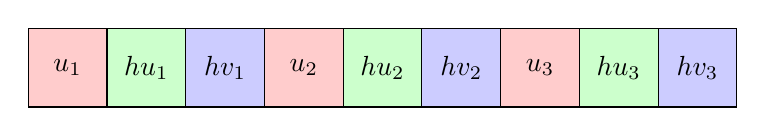
\begin{tikzpicture}
    \node[u]  (u1)  at (0, 0) {$u_1$};
    \node[hu] (hu1) at (1, 0) {$hu_1$};
    \node[hv] (hv1) at (2, 0) {$hv_1$};
    \node[u]  (u2)  at (3, 0) {$u_2$};
    \node[hu] (hu2) at (4, 0) {$hu_2$};
    \node[hv] (hv2) at (5, 0) {$hv_2$};
    \node[u]  (u3)  at (6, 0) {$u_3$};
    \node[hu] (hu3) at (7, 0) {$hu_3$};
    \node[hv] (hv3) at (8, 0) {$hv_3$};
  \end{tikzpicture}

  \vspace{0.5cm}

  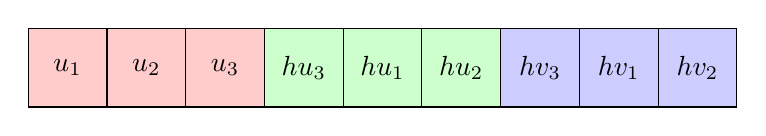
\begin{tikzpicture}
    \node[u]  (u1)  at (0, 0) {$u_1$};
    \node[u]  (u2)  at (1, 0) {$u_2$};
    \node[u]  (u3)  at (2, 0) {$u_3$};
    \node[hu] (hu3) at (3, 0) {$hu_3$};
    \node[hu] (hu1) at (4, 0) {$hu_1$};
    \node[hu] (hu2) at (5, 0) {$hu_2$};
    \node[hv] (hv3) at (6, 0) {$hv_3$};
    \node[hv] (hv1) at (7, 0) {$hv_1$};
    \node[hv] (hv2) at (8, 0) {$hv_2$};
  \end{tikzpicture}
  \caption{%
    (top) The memory layout of an array of structs as used in the reference
    simulator. (bottom) The memory layout of a struct of arrays as used in the
    vectorized simulator.
  }\label{fig:vec-to-arr}
\end{figure}

In addition to using flat arrays, we are also in the process of modifying loop
orderings, using \ttt{\#pragma ivdep} annotations, and generally rearranging
code in order to increase vectorization. We have already vectorized a fair
number of the loops, but some remain to be vectorized.
